The focus of this section is to present the broad overview of research within crosscutting concern mining we have acquired after classifying and categorizing primary studies. Moreover, we have used information drawn from this overview to answer this review study's research questions.

Aiming to show the frequencies of publication of all identified techniques for mining techniques for crosscutting concerns mining we have plotted a bubble plot, which is depicted in Figure~\ref{map}. Bubble plots are essentially two x-y scatter plots with bubbles in category intersections. The size of each bubble is determined by the number of primary studies that have been classified as belonging to the categories corresponding to the bubble coordinates. This visual summary provides a bird's-eye view that enables one to pinpoint which categories have been emphasized in past research along with gaps and opportunities for future research. 

In Figure~\ref{map} the facets we have used for organizing the map are the crosscutting concern mining techniques and year of publication. Based in this figure it is evident from observing it that we have found out 18 mining techniques for crosscutting concerns, as result we have answered the first part of the RQ$_1$. Based upon this bubble plot, we argue that the answer to second part of the RQ$_1$ is that Fan-In Analysis, Identifier Analysis and Dynamic Analysis are the techniques most used and Program Analysis Based, XScan-Concern-Peers, Data-Flow and Model Driven are the least used. More precisely, among the 62 primary studies included herein, 27 describe Fan-In Analysis, Identifier Analysis or Dynamic Analysis, respectively. In other hands, the techniques with less studies available in literature are Program Analysis Based, XScan-Concern-Peers, Data-Flow and Model Driven. Furthermore, it is argued that Fan-In Analysis, Identifier Analysis and Dynamic Analysis are evidence clusters (i.e., where there may be scope for more complete literature reviews to be undertaken). In contrast, Program Analysis Based, XScan-Concern-Peers, Data-Flow and Model Driven can be deemed as ``evidence desert'' (i.e., wherein better or new research is required). 

%According to this figure, a year-wise distribution of the CD, FI and DA reveals an increase in publication over time, most notable from 2006 to 2008. Moreover, Figure~\ref{frequencies_chart} depicts that the number of publication of these techniques have been stabilized in 2009 to 2011.

\begin{figure*}
\centering
  % Requires \usepackage{graphicx}
  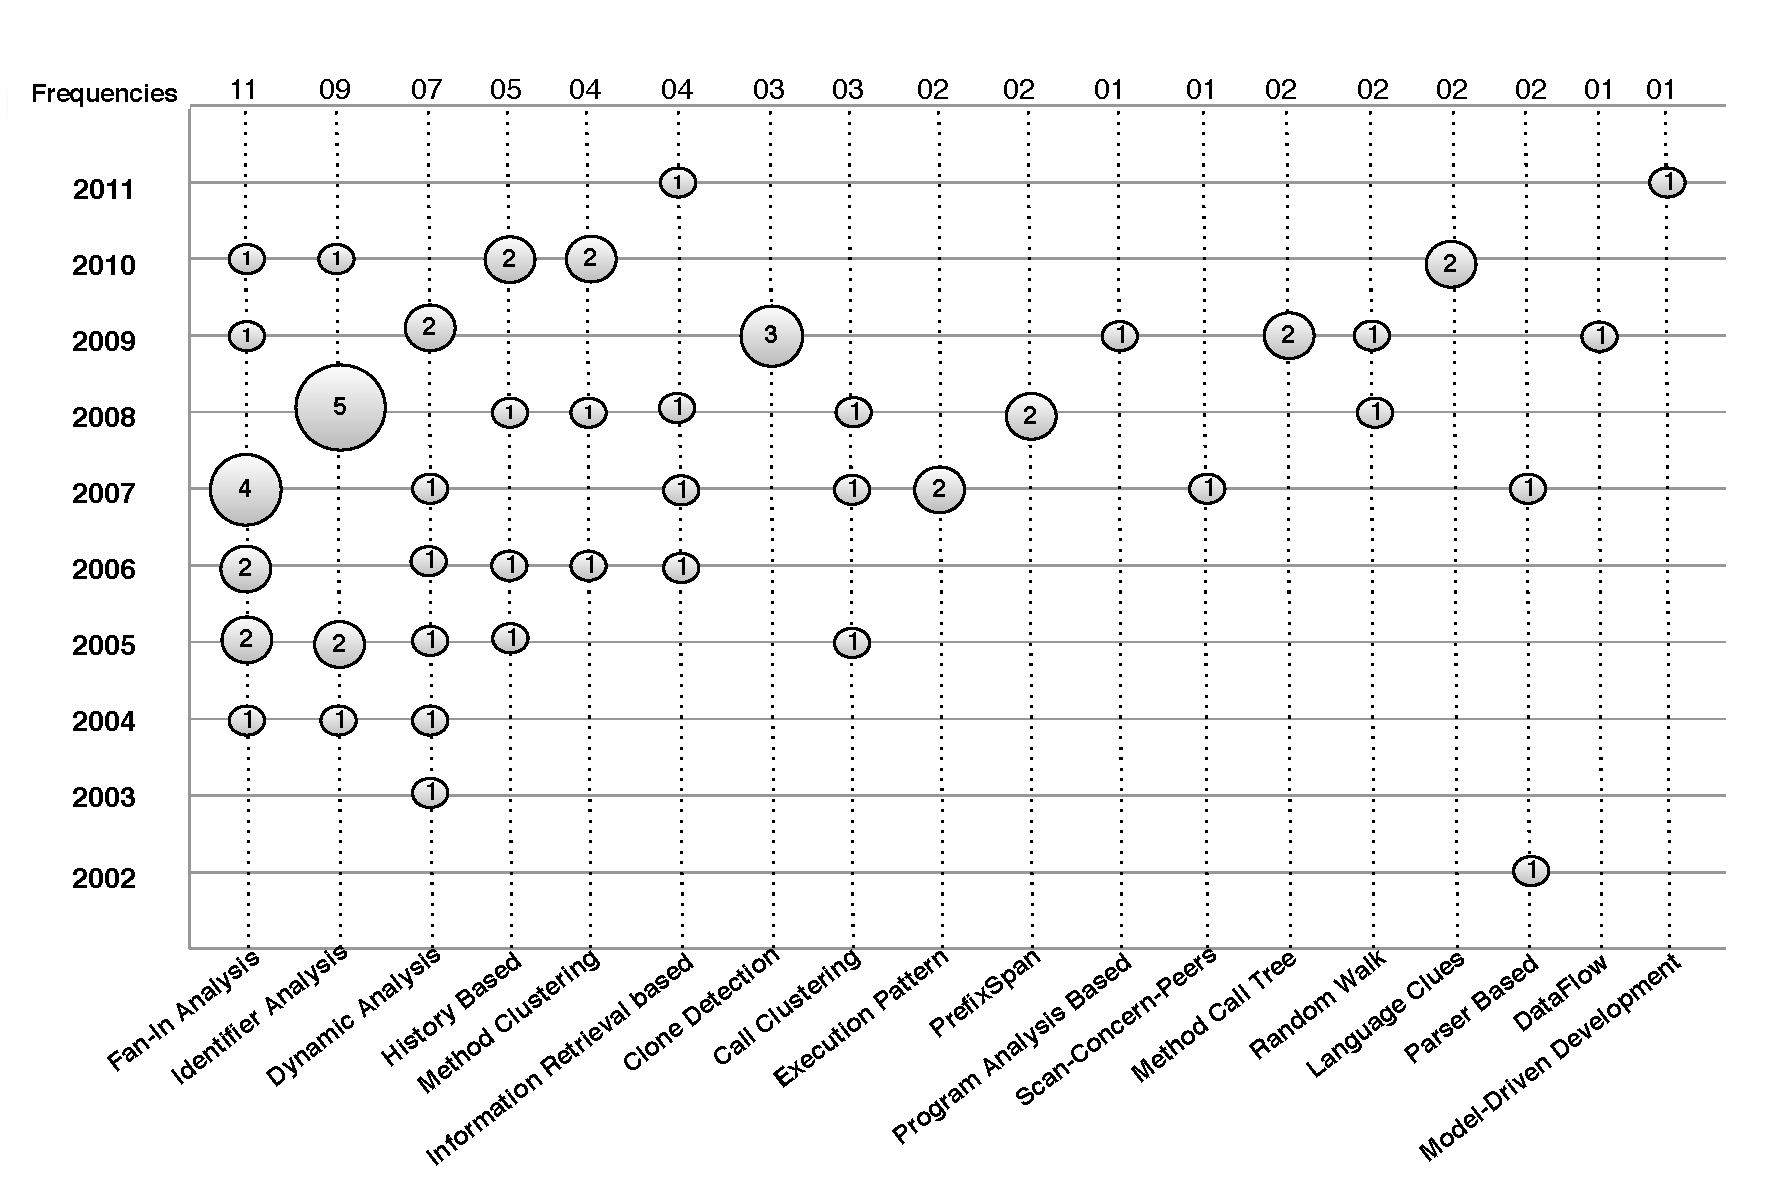
\includegraphics[width=14.5cm, height=7.3cm]{figuras/MapaDasTecnicas}
\caption{Map containing a year-wise distribution of publications on the all techniques found.}
\label{map}
\end{figure*} 

The majority of selected primary studies are published by IEEE, i.e., 20 primary studies. The others primary studies have been selected from ACM, Scopus and Springer, 18, 16 and 8, respectively. As for the publication types, we have selected primaries studies that have been published in conferences, workshops and journals. The majority of the primary studies are conference paper (37), followed by workshop (16) and journal (9).

%\begin{figure}[!h]
%\centering
  % Requires \usepackage{graphicx}
  %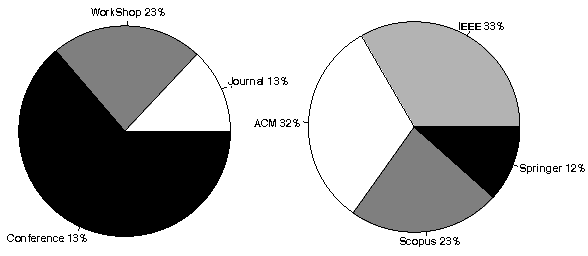
\includegraphics[scale=0.90]{figuras/PublicationTypeAndJounal2}
%\caption{Distribution of primary studies by publication type and distribution of primary studies by electronic database.}
%\label{publication_pie}
%\end{figure} 

\begin{figure}[!h]
\centering
  % Requires \usepackage{graphicx}
  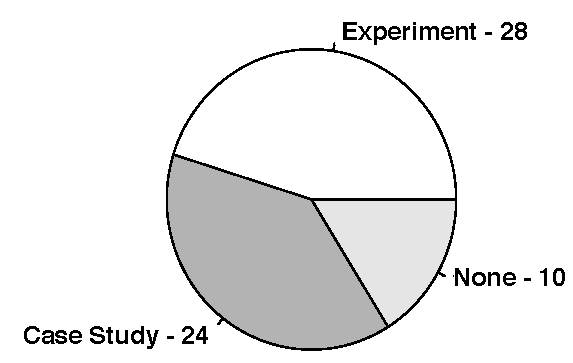
\includegraphics[scale=0.54]{figuras/pieChart}
\caption{Which empirical strategies have been employed.}
\label{empirical_strategies}
\end{figure} 


The way in which a technique is evaluated provides researchers and practitioners with useful information on the approach's quality, effectiveness, robustness, and practical applicability. Evaluating crosscutting concern mining techniques is difficult because defining the program elements that are relevant to a concern may be subjective. Despite this difficulty, researchers have devised some empirical strategies to assess them. 

Empirical strategies of software engineering techniques are classified as  experiment, case study and none~\cite{Wohlin}. In this context, we attempted to answer the RQ$_2$ by analyzing individually the 62 primary studies focus on gather which empirical strategies they have employed to validate the crosscutting concern mining techniques. In Figure~\ref{empirical_strategies} is depicted a pie chart wherein we have plotted the collected data. 

As can be seen, among the 62 primary studies, 52 have carried out at least one empirical strategy. More specifically, 28 have carried out experiments to validate their crosscutting concern mining techniques and 24 primary studies have employed some sort of case studies. Only 10 primary studies neither have carried out experiments/case studies nor have made evident the use of specific evaluation strategies in order to validate their mining crosscutting concern techniques. Among the 52 primary studies, i.e., studies which carried out some evaluation techniques, we identified 31 studies using JHotDraw~\cite{brantHot}, a widely used framework to validate their mining crosscutting concern techniques. It is worth highlighting that from the universe of 31 studies using JHotDraw, 6 of them were evaluated by using two most well-known relevance-based measures of effectiveness, recall and precision. Table~\ref{table_metrics} presents the techniques and tools of these 6 studies with the precision and recall metrics for a particular JHotDraw version and where some crosscutting concerns were mentioned.


\begin{table}[!t]\tiny
\centering
\caption{Precision and Recall for JHotDraw}
\begin{threeparttable}

\begin{tabular}{|c|l|c|c|c|c|}


\hline \multicolumn{6}{|c|}{Dynamic Analysis} \\ 
\hline {Ref.} & {Tool} &  {Precision} & {Recall} & {Concern} & {Version} \\
\cline{1-6}
\hline
&  &  &  &  &  \\
\multirow{2}{*}{\cite{Ceccato2009}}&\multirow{2}{*}{Dynamo}	&64\%           & 49\%     	  		&  	Undo	&\multirow{2}{*}{5.4}	\\
						& &100\%        & 26\%          	  & Persistence		&  		\\
&  &  &  &  &  \\						
\cline{1-6}
\hline \multicolumn{6}{|c|}{Concern Peers} \\ 
\hline {Ref.} & {Tool} &  {Precision} & {Recall} & {Concern} & {Version} \\
\cline{1-6}
&  &  &  &  &  \\
\multirow{5}{*}{\cite{Nguyen2011}}&\multirow{5}{*}{XScan}&90\%&93\%&Undo&\multirow{5}{*}{6} \\
&&100\%&89\%&Iterator & \\
&&100\%&93\%&Persistence & \\
&&97\%&100\%&Observer & \\
&&100\%&100\%&Visitor & \\
&  &  &  &  &  \\
\cline{1-6}
\hline \multicolumn{6}{|c|}{Method Clustering + Fan-In} \\ 
\hline {Ref.} & {Tool} &  {Precision} & {Recall} & {Concern} & {Version} \\
\cline{1-6}
&  &  &  &  &  \\
\multirow{5}{*}{\cite{Nguyen2011}}&\multirow{5}{*}{CBFA}&100\%&86\%&Undo&\multirow{5}{*}{6} \\
&&100\%&100\%&Iterator & \\
&&80\%&100\%&Persistence & \\
&&86\%&80\%&Observer & \\
&&86\%&100\%&Visitor & \\
&  &  &  &  &  \\
\cline{1-6}
\hline \multicolumn{6}{|c|}{Information Retrieval} \\ 
\hline {Ref.} & {Tool} &  {Precision} & {Recall} & {Concern} & {Version} \\
\cline{1-6}
&  &  &  &  &  \\
\multirow{4}{*}{\cite{Huang:2010:AMU:1901615.1902239}}&\multirow{4}{*}{MSAM} &\multirow{4}{*}{5\%} & \multirow{4}{*}{100\%}   	          &	 Undo	&\multirow{4}{*}{-} 			\\
& & & & Persistence &\\
& & & & Observer &\\
& & & & Command &\\
&  &  &  &  &  \\
\hline \multicolumn{6}{|c|}{Method Clustering} \\ 
\hline {Ref.} & {Tool} &  {Precision} & {Recall} & {Concern} & {Version} \\
\cline{1-6}
\hline
&  &  &  &  &  \\
\multirow{9}{*}{\cite{cojocar}}&&\multirow{9}{*}{87.5\%}& \multirow{9}{*}{-}&Observer &\multirow{9}{*}{5.2}\\
&   &&& &\\
&  Clustering &&& \textit{Consistent}&\\
&  Algorithms &&& \textit{Behaviour}&\\
&   &&& &\\
&   &&& \textit{Contract}&\\
&   &&& \textit{Enforcement}&\\
&   &&& &\\
&   &&& Command&\\
&  &  &  &  &  \\
\cline{1-6}
\hline \multicolumn{6}{|c|}{Call Clustering} \\ 
\hline {Ref.} & {Tool} &  {Precision} & {Recall} & {Concern} & {Version} \\
\cline{1-6}
&  &  &  &  &  \\
\multirow{9}{*}{\cite{Maisikeli:2009:AMU:1626886}}&\multirow{9}{*}{SOM}&\multirow{9}{*}{51\%}&\multirow{9}{*}{-}&Observer&\multirow{9}{*}{5.4} \\
&   &&& &\\
&  &  &  &\textit{Consistent} &  \\
&  &  &  &\textit{Behaviour}  &  \\
&   &&& &\\
&  &  &  &\textit{Contract}&  \\
&  &  &  &\textit{Enforcement}  &  \\
&   &&& &\\
&  &  &  &Command &  \\
&  &  &  &  &  \\
\cline{1-6}
\hline \multicolumn{6}{|c|}{Fan-In} \\ 
\hline {Ref.} & {Tool} &  {Precision} & {Recall} & {Concern} & {Version} \\
\cline{1-6}
&  &  &  &  &  \\
\multirow{5}{*}{\cite{Marin:2006:CFA:1174510.1174715}}&\multirow{5}{*}{FINT}&\multirow{5}{*}{30\%}&\multirow{5}{*}{-}&\textit{Consistent} &\multirow{5}{*}{5.4}\\
&  &  &  &\textit{Behavior}&  \\
&   &&& &\\
&  &  &  &\textit{Contract}&  \\
&  &  &  &\textit{Enforcement}  &  \\
&  &  &  &  &  \\
\cline{1-6}
\hline

\end{tabular}
\begin{tablenotes}
      \scriptsize
      \item *The values for MSAM were calculated using two thresholds, 0.4 for precision and 0.5 for recall.
    \end{tablenotes}
\end{threeparttable}
\label{table_metrics}
\end{table}


The data shown in Table~\ref{table_metrics} have useful information about how is the behavior in terms of precision and recall for different techniques regarding to JHotDraw concern. Note that there are some missing recall values because they were not reported. Recall is the proportion of relevant concern candidates that were discovered out of all concern candidates present in the source code. Thus a problem with calculating this metric, in a program under analysis, it is not known what the relevant concerns and code fragments are, except in an ideal case. In order to respond the RQ$_3$ take the persistence concern into account. It has a good precision value in most of the cases, that is, the percentage of relevant concern candidates in the set of all candidates reported was high. However, the recall value is uneven and this is a strong evidence that the universe of concern candidates used by each technique is not standardized. In other words, as shown in Table~\ref{table_metrics} usually there is a difference in the precision and recall metrics when different sorts of concerns are mined.

Based on the Table~\ref{table_metrics} we have answered the RQ$_4$. This table give us evidence that some techniques must be addressed to deal with certain kind of concerns instead of others. For instance, as shown in Table~\ref{table_metrics}, the best techniques to mine Persistence concern are XScan and CBFA, as they have a precision of 100\% - recall of 93\% and precision of 80\% - recall of 100\%, respectively. Similarly, the best techniques to mine Iterator concern are CBFA and XScan, since the former has both Precision and Recall of 100\% and the latter has a Precision of 100\% and Recall of 89\%.

In order to answer the RQ$_5$ we devised Table~\ref{table_conclusion} and Table~\ref{table_conclusion2}. Those tables show some candidate combinations of techniques described in Table~\ref{table_metrics}. Combining these techniques can improve precision and recall metrics. We consider that someone could implement and/or reuse the best of several techniques to create a better mining technique for crosscutting concerns. For instance, as we have stated earlier, XScan is the best technique to mine Persistence concern, since it  has a precision of 100\%, but it has a recall of 93\%. Therefore, maybe a solution to improve such recall, could be to combine other technique such as CFBA, which has a more reliable recall (100\%) as shown in Table~\ref{table_metrics}, i.e., first combination.

Also we stated that another solution to improve precision and recall metrics of techniques could be to combine the best techniques. For example, the second and the third combination illustrated in Table~\ref{table_conclusion} represent this solution. We established that maybe the percentage of Dynamo will be improved if someone combine it with either CBFA or XScan. Finally, the last alternative is to combine Dynamo and MSAM, since according to the Table~\ref{table_metrics}, the former has a good precision but it does not have a good recall, on the other side, the latter has a bad Precision but it has a good Recall. In the same way, Table~\ref{table_conclusion2}, shows two candidate combinations in order to improve precision and recall for Observer concern.

% Obviously, we have made this combinations just for example porpuse only because we do not take into account the system version but it is a factor that should be considered. The way that a specific concern is implemented may change between one version to another. 


\begin{table}[ht]\scriptsize
\begin{minipage}[b]{0.45\linewidth}
\centering
\captionof{table}{Combination for Persistence} 
\begin{tabular}{|c|c|}
\hline N & Combined Technique \\
\cline{1-2}
\nth{1}& CFBA + XScan	\\
\nth{2}& Dynamo + CBFA    \\
\nth{3}& Dynamo + XScan   \\
\nth{4}& MSAM + Dynamo   \\
\cline{1-2}
\end{tabular}
\label{table_conclusion}
\end{minipage}
\hspace{0.2cm}
\begin{minipage}[b]{0.45\linewidth}
\centering
\captionof{table}{Combination for Observer} 
\begin{tabular}{|c|c|}
\hline N & Combined Technique \\
\cline{1-2}
\nth{1}& MSAM + CBFA   \\
\multirow{2}{*}{\nth{2}}&MSAM + \\
&Clustering Algorithms \\
\cline{1-2}
\end{tabular}
\label{table_conclusion2}
\end{minipage}
\end{table}



%\begin{table}[!h]\scriptsize
%\centering
%\caption{Candidate Combination of Techniques for Persistence}
%
%
%\label{table_conclusion}
%\end{table}
%
%
%\begin{table}[!h]\scriptsize
%\centering
%\caption{Candidate Combination of Techniques for Observer}
%
%\label{table_conclusion2}
%\end{table}





